\documentclass[border=4pt]{standalone}
% Shared typography and colours for the standalone figures.
\usepackage{unicode-math}
\setmainfont{TeX Gyre Termes}
\setmathfont{TeX Gyre Termes Math}
\usepackage{tikz}
\usetikzlibrary{arrows.meta,positioning,calc,decorations.pathreplacing}
\usepackage{pgfplots}
\pgfplotsset{compat=1.18}

% One colour per element or subsystem. Record the mapping in
% the working repository conventions and use it identically in every figure.
\definecolor{elemA}{HTML}{1F5FA8}
\definecolor{elemB}{HTML}{B8461B}
\definecolor{elemC}{HTML}{2E7D32}
\definecolor{elemD}{HTML}{6A4C93}
\definecolor{frameline}{HTML}{555555}

\begin{document}
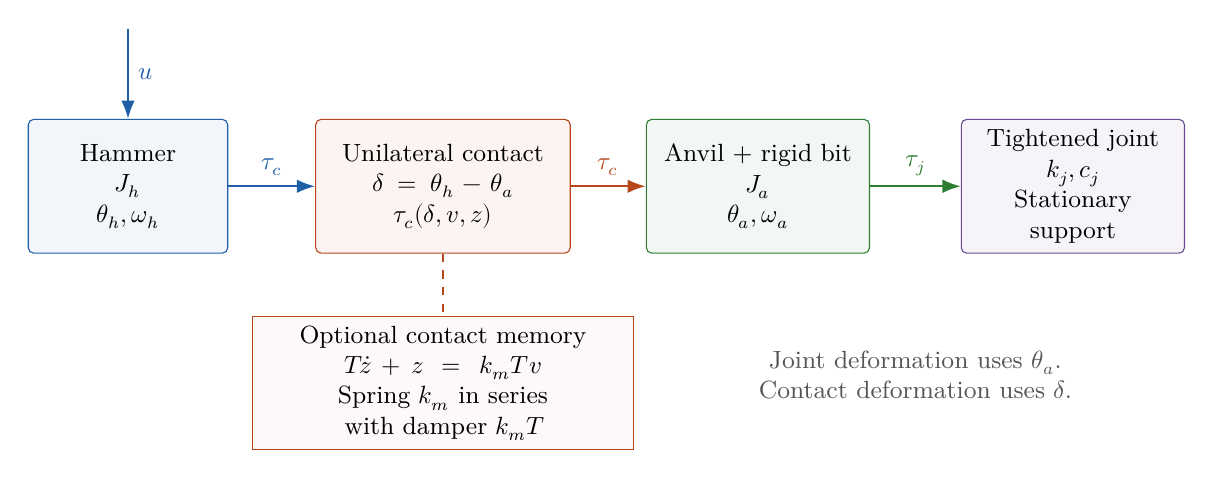
\begin{tikzpicture}[>=Latex,font=\small,
 box/.style={draw,rounded corners=2pt,align=center,minimum height=1.7cm},
 port/.style={->,thick}]
\node[box,draw=elemA,fill=elemA!6,text width=2.3cm] (h) at (0,0)
 {Hammer\\$J_h$\\$\theta_h,\omega_h$};
\node[box,draw=elemB,fill=elemB!6,text width=3.0cm] (c) at (4,0)
 {Unilateral contact\\$\delta=\theta_h-\theta_a$\\$\tau_c(\delta,v,z)$};
\node[box,draw=elemC,fill=elemC!6,text width=2.6cm] (a) at (8,0)
 {Anvil + rigid bit\\$J_a$\\$\theta_a,\omega_a$};
\node[box,draw=elemD,fill=elemD!6,text width=2.6cm] (j) at (12,0)
 {Tightened joint\\$k_j, c_j$\\Stationary support};
\draw[port,elemA] (h.east)--node[above] {$\tau_c$}(c.west);
\draw[port,elemB] (c.east)--node[above] {$\tau_c$}(a.west);
\draw[port,elemC] (a.east)--node[above] {$\tau_j$}(j.west);
\draw[port,elemA] (0,2)--node[right] {$u$}(h.north);
\node[draw=elemB,fill=elemB!3,align=center,text width=4.6cm] (branch) at (4,-2.5)
 {Optional contact memory\\$T\dot z+z=k_mTv$\\Spring $k_m$ in series with damper $k_mT$};
\draw[elemB,dashed] (c.south)--(branch.north);
\node[text=frameline,align=center] at (10,-2.4)
 {Joint deformation uses $\theta_a$.\\Contact deformation uses $\delta$.};
\end{tikzpicture}
\end{document}
